\section{Analysis register and statistical details}\label{supp:register}
Table~\ref{tab:register} lists every analysis and its inferential status: each primary analysis is a single prespecified test, secondary summaries are descriptive, and exploratory and post hoc analyses carry no $p$-values. Neither study met its success criterion, and the two studies are not pooled.

\begin{longtable}{P{0.23\linewidth}P{0.34\linewidth}P{0.34\linewidth}}
\caption{Analysis register.}\label{tab:register}\\
\toprule Analysis & Estimand & Inference\\\midrule\endfirsthead
\toprule Analysis & Estimand & Inference\\\midrule\endhead
Study 1 primary & Per-question $L-H$ answer F1, averaged over four chunkers (208 questions) & 20,000 question-bootstrap draws; 100,000 paired sign flips; one test.\\
Study 2 primary & Per-document $L-B$ response F1, averaged over four chunkers and three paired seeds (273 documents) & 20,000 family-bootstrap draws within domains; 100,000 family sign flips; one test.\\
Study 2 domains and seeds & Domain effects, equal-domain mean, seed spread and leave-one-seed-out values & Prespecified, descriptive.\\
Retrieval and operational outcomes & NDCG@4, span F1, exact match, cost & Prespecified, descriptive.\\
Pairwise contrasts and chunker breakdowns & All six method contrasts; all four chunkers & Exploratory, descriptive.\\
Evidence flow, overlap and associations & Specification dated 8 September 2026, 02:17:38 UTC & Exploratory; no $p$-values.\\
Validation grid on common grades & NDCG@4 of all 12 grid runs on both grade schemes & Post hoc, descriptive; one training seed.\\
Reserve exposure and design sensitivity & Study 1 exposure strata; normal-reference power and MDE calculations & Post hoc, descriptive; historical planning scenarios identified separately.\\\bottomrule
\end{longtable}

The Study~2 bootstrap resamples whole families within domains and computes the document-weighted statistic on each resample; the sign-flip test assigns one sign per family. There are 207 single-document families, 27 two-document families and one 12-document family in the SSA domain (235 families, 273 documents). Families are defined within domains by lowercased, trimmed titles with trailing numbered suffixes removed and whitespace normalized.

Specifically, let $\mathcal{F}_h$ be the set of families in domain $h$, $C_f$ the documents in family $f$, and $\Delta_d$ the document's mean $L-B$ response-F1 difference over the 12 chunker--seed cells. Each draw independently samples $|\mathcal{F}_h|$ families with replacement within each domain. If $w_f^*$ is the resulting multiplicity of family $f$, the executed bootstrap statistic is
\begin{equation}
\widehat{\Delta}^{\,*}=\frac{\sum_h\sum_{f\in\mathcal{F}_h}w_f^*\sum_{d\in C_f}\Delta_d}{N^*},\qquad
N^*=\sum_h\sum_{f\in\mathcal{F}_h}w_f^*|C_f|.
\end{equation}
The denominator is the resampled document count $N^*$, which varies with the sampled family sizes; it is not fixed at 273. Each occurrence of a document has equal weight, rather than each family having equal weight. Domain family counts are fixed by stratification, but domain document counts can vary. For the sign-flip test, the denominator remains 273 and one random sign multiplies all document differences in a family.

The analysis random seeds are 20260907 (bootstrap) and 20260908 (sign flips) for Study~1, and 20260922 and 20260923 for Study~2; they are separate from the training seeds. The success criterion in both studies is an observed mean improvement of at least $+1$ F1 point with two-sided $p<0.05$. The Study~2 interval ($\StwoLow$ to $\StwoHigh$ points) excludes $+1$; no equivalence test was planned.

\paragraph{Training-seed scope.} The family bootstrap conditions on the three paired sets of trained adapters. It does not cover uncertainty from drawing new training seeds. We report the individual seed effects, their sample standard deviation and leave-one-seed-out means descriptively. No seed-general confidence interval is claimed: combining a document-bootstrap interval with a three-seed variance estimate would require additional assumptions about dependence and the target population.

\paragraph{Planning and retrospective sensitivity.} The pre-execution Study~2 planning record used a TechQA development proxy: the per-question generic-reranker minus hybrid F1 difference, averaged over four chunkers ($n=200$; SD 0.06062 on the 0--1 F1 scale, or 6.06 points). It gave normal-reference power of 77.8\% under independence and 70.0\% under an assumed family ICC of 0.3 for a true $+1$-point effect. These calculations concern the two-sided significance requirement alone, use a different dataset and contrast, and do not estimate the probability of satisfying the full compound success rule.

Table~\ref{tab:sensitivity} reports these sensitivity calculations; neither study's frozen decision rule is changed. For an assumed standard error $s$, the significance-only calculation uses $\Pr(|Z+\delta/s|>1.96)$; the compound rule uses the positive-effect threshold $t=\max(1,1.96s)$, with $t$ and $s$ in F1 points, and approximate power $1-\Phi((t-\delta)/s)$. Thus its 80\% minimum detectable effect (MDE) is $t+\Phi^{-1}(0.8)s$. Study~1's retrospective $s$ is the SD of its 208 question differences divided by $\sqrt{208}$ (0.526 F1 points). Study~2 uses the standard deviation of its reproduced 20,000 frozen family-bootstrap replicates (0.218 points); the reproduction recovers the reported percentile interval. These normal-reference approximations are not exact power calculations for the sign-flip tests, and the retrospective rows condition on the observed variance and trained adapters. In particular, an observed-effect threshold of $+1$ point yields only about 50\% probability of crossing that threshold when the true effect equals it, even when the significance-only power is high.
\begin{longtable}{P{0.36\linewidth}rrrr}
\caption{Normal-reference sensitivity. MDEs are F1 points at 80\% power; power columns assume a true $+1$-point effect. Historical planning and retrospective approximations are distinct.}\label{tab:sensitivity}\\
\toprule Scenario & \multicolumn{2}{c}{MDE (points)} & \multicolumn{2}{c}{Power (\%)}\\
 & $p$ only & Compound & $p$ only & Compound\\\midrule\endfirsthead
\toprule Scenario & \multicolumn{2}{c}{MDE (points)} & \multicolumn{2}{c}{Power (\%)}\\
 & $p$ only & Compound & $p$ only & Compound\\\midrule\endhead
Study 1, retrospective & 1.47 & 1.47 & 47.7 & 47.7\\
Study 2, planning, independent & 1.03 & 1.31 & 77.8 & 50.0\\
Study 2, planning, ICC 0.3 & 1.13 & 1.34 & 70.0 & 50.0\\
Study 2, retrospective bootstrap scale & 0.61 & 1.18 & 99.6 & 50.0\\\bottomrule
\end{longtable}

\paragraph{Secondary testing.} An earlier planning proposal described $L-U$, $B-U$, $U-H$, $L-H$ and $B-H$ contrasts with one Holm adjustment. Both frozen protocols (preflight v1 and the final pre-execution v2) instead list secondary summaries without that hypothesis family. The executed configuration has SHA-256 \nolinkurl{5820ef0c0901689b46e155ab0c2e09d818698a3652a75e3071804ea11c835cb2}; the execution freeze is recorded at 7 September 2026, 03:38:34 UTC, before comparative Doc2Dial outcomes existed. The final protocol has SHA-256 \nolinkurl{87cbc55f57526fe31af3931df4157a2216db146038376d42a1b66a1844373a6a}. Secondary outcomes are therefore reported descriptively. No written rationale for dropping the Holm family was retained, and no tests were reclassified after results were seen.

\section{Implementation details}\label{supp:impl}
In the study protocol and the released files, L is named ``evidence-specific'' (condition E), and the Study~1 system ``evidence-aware''; we use L throughout.

\subsection{Data}
Study~1 uses the NVIDIA TechQA-RAG-Eval training distribution at revision \nolinkurl{0b5bbc84b7f07d6d09d063130e90b716d8d4a32a}, split 200/200/208 into training, validation and reserve questions. The split sorts the 608 eligible question identifiers by the SHA-256 digest of the salt \nolinkurl{eaai-phase2-techqa-v1}, a NUL byte and the identifier (then by identifier) and assigns the first 200 to training, the next 200 to validation and the last 208 to reserve. A retrospective recomputation of this rule from the identifier list reproduces all 608 saved assignments. The original TechQA paper \citep{castelli2020} describes the underlying task; its split sizes do not apply to this distribution. Study~2 uses the official Doc2Dial v1.0.1 archive (\url{https://doc2dial.github.io/file/doc2dial_v1.0.1.zip}; SHA-256 \nolinkurl{94499fa5259f69018d2458cb948552e7a05f424711a95a562bb9e816a515dc23}) \citep{feng2020}; the one-transition-per-document conversion is specific to this study.

All 488 Doc2Dial documents are searchable, and the evaluation set has 51 DMV, 77 SSA, 50 student-aid and 95 VA cases. Eligibility starts from documents represented in the official validation dialogues: a user turn must be followed immediately by an agent turn with a nonblank utterance and at least one grounding reference. Every one of the 273 validation documents has an eligible transition. Within each document, the transition minimizing SHA-256 of \texttt{salt|domain|document\_id|dialogue\_id|user\_turn\_id} is chosen; the fixed salt is \nolinkurl{eaai-phase4-doc2dial-one-case-per-document-v1-20260906}. Thus the difference between 488 searchable and 273 evaluated documents reflects corpus versus validation-dialogue membership, not selection on comparative outcomes. The query serializes the dialogue history up to the selected user turn, one turn per line, as the uppercase role, a colon and a space, then the utterance. Later turns, the target utterance, gold identifiers, offsets, grounding spans, grades and the reading-comprehension answer field are not used at inference. This supplement reproduces no question, candidate or generated-response text. Exact selection records and per-record outputs are not in the current companion, reflecting its release scope (Section~\ref{supp:repro}).

\subsection{Models and configuration}
Table~\ref{tab:models} lists the pinned components.
\begin{longtable}{P{0.27\linewidth}P{0.65\linewidth}}
\caption{Pinned models and revisions.}\label{tab:models}\\
\toprule Component & Model and revision\\\midrule\endfirsthead
\toprule Component & Model and revision\\\midrule\endhead
Reranker & Qwen/Qwen3-Reranker-0.6B; \nolinkurl{e61197ed45024b0ed8a2d74b80b4d909f1255473}\\
Generator & Qwen/Qwen3.5-9B; \nolinkurl{1eb6d84878284892ecfd4c3fb760ffbf34548234}\\
Dense embedding & BAAI/bge-small-en-v1.5; \nolinkurl{5c38ec7c405ec4b44b94cc5a9bb96e735b38267a}\\
Chunking tokenizer & sentence-transformers/all-MiniLM-L6-v2; \nolinkurl{1110a243fdf4706b3f48f1d95db1a4f5529b4d41}\\\bottomrule
\end{longtable}
Each dense and BM25 channel retrieves 20 candidates. Reciprocal-rank fusion over their union adds $0.6/(60+r_{\rm dense})$ and $0.4/(60+r_{\rm sparse})$, with a missing channel rank contributing zero, then retains the top 20; each method returns four passages. Exact fused-score ties preserve insertion order: dense rank order first, followed by previously unseen sparse candidates in sparse rank order. Reranker ties use descending reranker score, ascending fused rank and ascending chunk identifier. The dense query prefix is ``Represent this sentence for searching relevant passages: ''. The pinned embedding configuration sets a 512-token maximum and lowercasing. SentenceTransformers 3.4.1 tokenizes the combined prefix/query string with \texttt{longest\_first} truncation; with the tokenizer's default right truncation, overlength inputs retain the beginning and discard the suffix, within 512 total tokens including special tokens. This can remove later dialogue turns, including the selected user turn; the runner implements no turn-aware shortening rule. This behavior is derived from the immutable model configuration and pinned library source, not a replay of per-record tokenization.\footnote{See the \href{https://huggingface.co/BAAI/bge-small-en-v1.5/blob/5c38ec7c405ec4b44b94cc5a9bb96e735b38267a/sentence_bert_config.json}{pinned embedding configuration}, \href{https://github.com/UKPLab/sentence-transformers/blob/v3.4.1/sentence_transformers/models/Transformer.py\#L427-L464}{SentenceTransformers 3.4.1 tokenization}, and \href{https://github.com/huggingface/transformers/blob/v5.16.1/src/transformers/tokenization_utils_base.py\#L882-L883}{Transformers 5.16.1 defaults}.}

Study~2 LoRA uses rank 16, alpha 32, dropout 0.05, all linear target modules and no bias adaptation. AdamW uses weight decay 0.01, warmup over 10\% of the update budget (rounded up) and gradient-norm clipping at 1.0. Two groups per device and two accumulation steps give four groups per update; the maximum pair length is 512 tokens. Groups are shuffled with seed equal to the training seed plus $1000003\times$epoch, and each epoch is completed before reshuffling until the draw budget is reached.

The grid (one seed, two learning rates, three update budgets per method) produces 192,000 validation candidate scores across 12 validation runs. Configuration selection averages B's and L's validation NDCG@4 over all validation questions and chunkers; each method's validation NDCG uses its own training grades (binary for B, three-level for L). The selected shared learning rate is $10^{-4}$ with 227 updates. The pre-frozen lookup maps 227, 454 and 681 grid updates to 431, 862 and 1,293 refit updates; no derivation formula was preserved in the located records. Retrospectively, these values equal $k\lceil 907/4\rceil$ and $k\lfloor 1{,}725/4\rfloor$ for $k=1,2,3$, where 907 and 1,725 are Study~1's surviving training and refit groups (reported below). The lookup therefore corresponds arithmetically to one to three Study~1 epochs at four groups per update, matching Study~1's one-to-three-epoch grid. Because the rounding direction differs (up for training, down for refits) and no located record states this rule, the correspondence is a reconstruction, not the documented derivation. All six final B/L refits use 431 updates. Retrospective inspection of the complete saved grid shows that independent selection on each method's own grades would retain $10^{-4}$/227 for B but choose $5\times10^{-5}$/227 for L (0.817378 versus 0.810474 at the shared choice). The corresponding independently selected L transfer experiment was not run. Generation uses bfloat16, greedy decoding (temperature zero, one beam), no thinking, a 1,536-token input limit, a 512-token output limit and batch size four.

\subsection{Prompts}\label{supp:prompts}
The reranker scores each query--passage pair with the Qwen3-Reranker template below; the score is the final-token logit for ``yes'' minus that for ``no''. In Study~2 the query is the serialized dialogue history.
\begin{lstlisting}
<|im_start|>system
Judge whether the Document meets the requirements based on the Query and the Instruct provided. Note that the answer can only be "yes" or "no".<|im_end|>
<|im_start|>user
<Instruct>: Given a technical-support question, rank passages by whether they contain sufficient evidence to answer it.
<Query>: {query}
<Document>: {passage}<|im_end|>
<|im_start|>assistant
<think>

</think>

\end{lstlisting}
The generator receives two chat messages, rendered with the model's chat template with thinking disabled. The context lists the top four passages in ranked order as \texttt{[1]}~\ldots~\texttt{[4]}, separated by blank lines. If the prompt exceeds 1,536 tokens, binary search finds the longest decoded token prefix of this concatenated context that fits, preserving the complete query/history and fixed prompt. This removes the context suffix, may cut a passage midway, and gives earlier ranked passages priority; no early dialogue turn is evicted. If the query and fixed prompt alone cannot fit, the function raises an error. The same prompt function is used by the Study~1 generation code. Reranker inference is separate: it reserves the Qwen prefix and suffix tokens and tokenizes the combined instruction/query/document body with \texttt{truncation=True} to the remaining 512-token budget. The runner sets padding side but leaves truncation side to the pinned tokenizer default; the pinned tokenizer configuration sets none, so the library's right-side default applies. Because the body is ordered instruction, query, document, an overlength pair loses the end of the passage first and, for a long enough dialogue history, the whole passage or the end of the query. Training pruned pairs over 512 tokens instead, so inference truncates inputs of a kind that training excluded. The numbers of overlength dense queries and reranker pairs were not recorded; counting them requires replaying the pinned tokenizers on the saved queries and candidate pools.
\begin{lstlisting}
system: You are a grounded question answering assistant. Use only the provided context. Give a concise but complete answer containing the information needed to resolve the question. Do not explain your reasoning or add citations. If the answer is not fully supported, reply with exactly 'unanswerable'.
user: Answer the following question using only the context.

Question: {question}

Context passages:
{context}

Return only the final answer.
\end{lstlisting}
Before scoring, outputs are stripped of a leading passage marker (\texttt{[n]}) and prefixes such as ``Answer:'' or ``The answer is''.

\subsection{Validation grid on common grades (post hoc)}\label{sec:validationgrid}
During model selection, each method's validation NDCG@4 used its own training grades, so B and L were not scored on the same scale. After the study, we re-scored the saved validation rankings of all 12 grid runs on both grade schemes, using the frozen validation labels and the saved reranker scores; no model was retrained or invoked. A separate retrospective recomputation reproduces all 12 recorded own-grade selection values from the saved scores and verifies their file hashes against the run summaries (maximum numerical discrepancy $1.2\times10^{-16}$). Table~\ref{tab:validationgrid} reports the results, with the hybrid order as a reference.

On L's own grades, L is below B at the selected configuration (0.810 vs 0.824; per-question difference $-0.013$, 95\% CI $-0.026$ to $-0.001$ from 10,000 paired question-bootstrap draws with seed 20261007; L lower on 75 and higher on 42 of 200 questions). L is also lower in five of the six matched configurations; the exception is $5\times10^{-5}$ with 227 updates (L 0.817, B 0.799), the only grid configuration in which L exceeds B on both grade schemes (0.826 vs 0.809 on B grades). Moving from $5\times10^{-5}$ to $10^{-4}$ at 227 updates raised B's own-grade score by 0.029 and lowered L's by 0.007, so the shared average favored B's optimum. At $5\times10^{-5}$, L's own-grade score falls as updates increase (0.817, 0.799, 0.790), which is consistent with, but does not demonstrate, sensitivity to the additional passes over its smaller inventory. On B's grades, the selected-configuration difference is $-0.021$ ($-0.033$ to $-0.008$). This analysis was not part of the protocol and uses a single training seed.
\begin{table}[htbp]\centering\small
\caption{Study 2 development grid: TechQA validation NDCG@4 for every run, scored on both grade schemes (post hoc, one training seed, 200 questions). Model selection used each method's own grades (B column for B runs, L column for L runs); the selected configuration is $10^{-4}$ with 227 updates.}\label{tab:validationgrid}
\begin{tabular}{lrrrr}\toprule
Method & LR & Updates & B grades & L grades\\\midrule
H (hybrid order) & -- & -- & 0.780 & 0.767\\
B & $5\times10^{-5}$ & 227 & 0.809 & 0.799\\
B & $5\times10^{-5}$ & 454 & 0.822 & 0.810\\
B & $5\times10^{-5}$ & 681 & 0.817 & 0.805\\
B & $10^{-4}$ & 227 & 0.838 & 0.824\\
B & $10^{-4}$ & 454 & 0.831 & 0.819\\
B & $10^{-4}$ & 681 & 0.835 & 0.821\\
L & $5\times10^{-5}$ & 227 & 0.826 & 0.817\\
L & $5\times10^{-5}$ & 454 & 0.804 & 0.799\\
L & $5\times10^{-5}$ & 681 & 0.797 & 0.790\\
L & $10^{-4}$ & 227 & 0.817 & 0.810\\
L & $10^{-4}$ & 454 & 0.790 & 0.786\\
L & $10^{-4}$ & 681 & 0.800 & 0.798\\
\bottomrule\end{tabular}\end{table}
\FloatBarrier

\subsection{Training groups and Study 1 differences}
In Study~2, label-blind deduplication precedes grouping and removes normalization-empty candidates. Within each question/normalized-text key, representatives minimize fused rank, then chunker priority (fixed-128, fixed-254, recursive-254, sentence-254), then chunk identifier. Near-identical passages remain distinct if their normalized texts differ. Candidates are then ordered by fused rank and chunk identifier, and each highest-grade positive forms a group with the first up to seven lower-grade candidates. If a grade-2 candidate exists, grade-1 candidates are eligible negatives; otherwise L falls back to grade-1 positives. Pairs include the complete Qwen template: positives over 512 tokens remove their groups; negatives over 512 are pruned individually, with no replacement. A group needs an in-limit positive and at least one surviving negative. Highest grade is determined before pair pruning; groups are not rebuilt with grade-1 positives if every literal-positive group is removed. The loss is group-level cross entropy with the positive at index zero, using yes-minus-no logits at temperature one. Weighting groups equally does not weight questions equally.

Table~\ref{tab:groupaudit} summarizes a retrospective audit of the frozen usable group inventories. L's usable questions are a subset of B's: there are two B-only training questions and three B-only refit questions. Most L groups use grade-1 fallback rather than literal-positive supervision. Training B groups per retained question range from 2 to 59 (median 8), versus 1 to 53 for L (median 3); refit ranges are 1--59 (median 8) and 1--53 (median 3). Table~\ref{tab:trainingcost} reports further exposure and cost information.
\begin{table}[htbp]\centering\small
\caption{Retrospective audit of Study~2's frozen usable group inventories. Questions are those yielding at least one surviving group. Grade columns count group positives; passes are total group draws divided by inventory size at the selected budget, not equal question exposure.}\label{tab:groupaudit}
\begin{tabular}{llrrrrr}\toprule
Split & Method & Questions & Groups & Grade 2 & Grade 1 & Passes\\\midrule
Train (200) & B & 189 & 2,103 & 0 & 2,103 & 0.432\\
 & L & 187 & 943 & 212 & 731 & 0.963\\
Refit (400) & B & 379 & 4,019 & 0 & 4,019 & 0.429\\
 & L & 376 & 1,799 & 430 & 1,369 & 0.958\\\bottomrule
\end{tabular}\end{table}

Grade-2 positives account for 22.5\% of L's training groups and 23.9\% of its refit groups. Within these grade-2 groups, grade-1 passages occupy 759 of 1,466 negative positions in training (51.8\%) and 1,551 of 2,971 positions in refitting (52.2\%). At least one grade-1 negative appears in 186 of 212 grade-2 training groups and 361 of 430 refit groups. Position counts repeat the shared negatives once per positive group and describe the full usable inventory, not realized optimizer draws. Four raw out-of-document grade-2 candidate rows across two questions produce three usable literal-positive groups, in both the training and refit inventories. Raw candidate counts include cross-chunker duplicates. These audits quantify coupled mechanisms without isolating their causal effects.

At 227 updates, 908 group draws correspond to 0.432 B and 0.963 L training passes; at 454 updates these are 0.864 and 1.926, and at 681 updates 1.295 and 2.889. The selected refits draw 1,724 groups (431 updates), corresponding to 0.429 B and 0.958 L passes.

Study~1's earlier pipeline chooses normalized-text duplicate representatives by higher grade first, then lower fused rank, chunker priority and chunk identifier; it deletes the whole group when the positive or any negative exceeds 512 tokens. Of 995 saved training groups, 907 survive; of 1,903 refit groups, 1,725 survive. Of 191 training questions represented before length filtering, 178 remain, and one question supplies up to 53 surviving groups. Study~1 used MS-SWIFT and an epoch grid; Study~2 explicitly batches intact groups under fixed update budgets and uses pair-level pruning fixed before execution. The studies therefore evaluate different training pipelines.

\subsection{Metric definitions}
Answer normalization lowercases text, removes ASCII punctuation and the articles ``a'', ``an'' and ``the'', and collapses whitespace. Token F1 uses multiset overlap and takes the maximum over reference answers where several exist; two empty strings score one, and one empty string scores zero. Exact match tests normalized equality. For TechQA supervision, literal matching tests a complete nonempty normalized reference as a contiguous token sequence. If a reference is longer than a passage or split across passages, partial containment does not yield grade~2; any complete alternative reference may qualify. In the executed Doc2Dial retrieval grading function, the same normalization is followed instead by a character-substring test for any nonempty annotated grounding span, which can match within a normalized word. Neither implementation requires gold-document membership for grade~2. Neither applies Unicode normalization, casefolding or fuzzy matching. These literal tests are deterministic proxies rather than semantic sufficiency labels. For returned grades $g_i$ and pool grades sorted descending $g_i^*$,
\[
 \mathrm{DCG}@4=\sum_{i=1}^{4}\frac{2^{g_i}-1}{\log_2(i+1)},\qquad
 \mathrm{IDCG}@4=\sum_{i=1}^{4}\frac{2^{g_i^*}-1}{\log_2(i+1)}.
\]
NDCG@4 is their ratio when IDCG@4 is positive and zero otherwise; zero-IDCG cells remain in the averaging denominator. The ideal uses the best four of the complete 20-candidate pool. Study~2 evaluation methods share that pool and three-level grading within each query--chunker cell, whereas development selection used method-specific grades. In Doc2Dial, agent-response F1 and grounding-span F1 are separate targets.

\section{Complete Study 2 results}\label{supp:study2}
Tables~\ref{tab:domainmethods}--\ref{tab:seedmethods} report every method by domain, chunker and training seed; Table~\ref{tab:chunkers} gives the $L-B$ effect by chunker, Table~\ref{tab:pairwise} all six method contrasts, and Figure~\ref{fig:methodmeans} the overall method means. H and U do not depend on the training seed and are not repeated in the seed table. Exact match is near zero for all methods and is omitted from the breakdowns; it is available in the released CSV files.
\begin{table}[htbp]\centering\small
\caption{Study 2 method means by domain. F1 in points; NDCG@4 and span-at-4 on the 0--1 scale. Span at 4 is the fraction of cells whose top four passages contain an annotated grounding span literally.}\label{tab:domainmethods}
\begin{tabular}{lrrrrr}\toprule
Domain & Method & Resp. F1 & Span F1 & NDCG@4 & Span at 4\\\midrule
DMV & H & 26.95 & 24.39 & 0.652 & 0.706\\
DMV & U & 27.71 & 26.92 & 0.726 & 0.789\\
DMV & B & 28.27 & 26.10 & 0.726 & 0.788\\
DMV & L & 27.64 & 25.78 & 0.656 & 0.747\\
SSA & H & 20.97 & 21.71 & 0.571 & 0.565\\
SSA & U & 21.77 & 21.84 & 0.586 & 0.594\\
SSA & B & 20.86 & 21.54 & 0.611 & 0.619\\
SSA & L & 20.75 & 21.35 & 0.525 & 0.592\\
Student aid & H & 22.68 & 21.04 & 0.686 & 0.675\\
Student aid & U & 22.37 & 20.40 & 0.751 & 0.725\\
Student aid & B & 22.66 & 20.87 & 0.737 & 0.712\\
Student aid & L & 22.48 & 20.65 & 0.675 & 0.700\\
VA & H & 24.33 & 23.34 & 0.693 & 0.697\\
VA & U & 24.77 & 24.06 & 0.710 & 0.726\\
VA & B & 25.10 & 24.32 & 0.706 & 0.725\\
VA & L & 24.98 & 24.42 & 0.625 & 0.677\\
\bottomrule\end{tabular}\end{table}
\FloatBarrier
\begin{table}[htbp]\centering\small
\caption{Study 2 method means by chunker. F1 in points; NDCG@4 and span-at-4 on the 0--1 scale. Span at 4 is the fraction of cells whose top four passages contain an annotated grounding span literally.}\label{tab:chunkermethods}
\begin{tabular}{lrrrrr}\toprule
Chunker & Method & Resp. F1 & Span F1 & NDCG@4 & Span at 4\\\midrule
fixed\_128 & H & 23.71 & 22.81 & 0.589 & 0.509\\
fixed\_128 & U & 24.46 & 24.06 & 0.647 & 0.601\\
fixed\_128 & B & 24.77 & 23.80 & 0.653 & 0.604\\
fixed\_128 & L & 24.51 & 23.74 & 0.558 & 0.565\\
fixed\_254 & H & 23.41 & 22.38 & 0.669 & 0.696\\
fixed\_254 & U & 23.37 & 22.73 & 0.714 & 0.740\\
fixed\_254 & B & 23.76 & 22.67 & 0.707 & 0.735\\
fixed\_254 & L & 23.72 & 23.03 & 0.619 & 0.697\\
recursive\_254 & H & 23.73 & 22.84 & 0.664 & 0.667\\
recursive\_254 & U & 24.22 & 23.00 & 0.683 & 0.674\\
recursive\_254 & B & 24.03 & 23.49 & 0.692 & 0.686\\
recursive\_254 & L & 23.04 & 22.34 & 0.621 & 0.659\\
sentence\_254 & H & 23.43 & 22.58 & 0.676 & 0.758\\
sentence\_254 & U & 24.08 & 23.41 & 0.698 & 0.788\\
sentence\_254 & B & 23.63 & 22.98 & 0.704 & 0.791\\
sentence\_254 & L & 24.04 & 23.35 & 0.648 & 0.759\\
\bottomrule\end{tabular}\end{table}
\FloatBarrier
\begin{table}[htbp]\centering\small
\caption{Study 2 method means by seed. F1 in points; NDCG@4 and span-at-4 on the 0--1 scale. Span at 4 is the fraction of cells whose top four passages contain an annotated grounding span literally.}\label{tab:seedmethods}
\begin{tabular}{lrrrrr}\toprule
Seed & Method & Resp. F1 & Span F1 & NDCG@4 & Span at 4\\\midrule
20260904 & B & 23.61 & 23.02 & 0.697 & 0.708\\
20260904 & L & 23.96 & 23.21 & 0.615 & 0.678\\
20260905 & B & 24.42 & 23.43 & 0.681 & 0.700\\
20260905 & L & 23.94 & 23.08 & 0.626 & 0.679\\
20260906 & B & 24.11 & 23.25 & 0.689 & 0.705\\
20260906 & L & 23.58 & 23.06 & 0.595 & 0.655\\
\bottomrule\end{tabular}\end{table}

\begin{table}[htbp]\centering\small
\caption{Study 2 $L-B$ response-F1 difference by chunker (points; exploratory).}\label{tab:chunkers}
\begin{tabular}{lr}\toprule
Chunker & $L-B$ F1\\\midrule
fixed\_128 & $-$0.26\\
fixed\_254 & $-$0.04\\
recursive\_254 & $-$0.99\\
sentence\_254 & $+$0.41\\
\bottomrule\end{tabular}\end{table}
\FloatBarrier
\begin{table}[htbp]\centering\small
\caption{All six Study 2 method contrasts (exploratory). F1 differences in points; NDCG@4 differences on the 0--1 scale. Only $L-B$ response F1 is the confirmatory test.}\label{tab:pairwise}
\begin{tabular}{lrrr}\toprule
Contrast & Resp. F1 & Span F1 & NDCG@4\\\midrule
U $-$ H & $+$0.46 & $+$0.64 & $+$0.036\\
B $-$ H & $+$0.48 & $+$0.58 & $+$0.039\\
L $-$ H & $+$0.26 & $+$0.46 & $-$0.038\\
B $-$ U & $+$0.02 & $-$0.06 & $+$0.003\\
L $-$ U & $-$0.20 & $-$0.18 & $-$0.074\\
L $-$ B & $-$0.22 & $-$0.12 & $-$0.077\\
\bottomrule\end{tabular}\end{table}
\FloatBarrier
\begin{figure}[htbp]\centering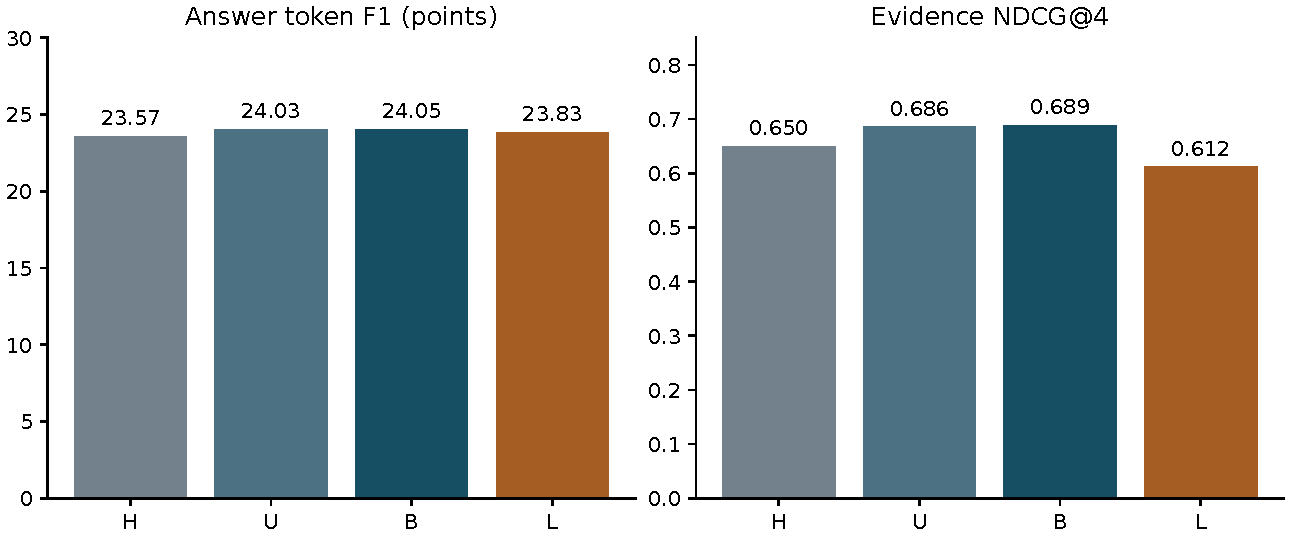
\includegraphics[width=\linewidth]{figures/study2_methods.pdf}
\caption{Study 2 method means: answer token F1 in points (left) and evidence NDCG@4 (right). H/U: 1,092 records each; B/L: 3,276 each over three training seeds.}\label{fig:methodmeans}\end{figure}\FloatBarrier

\clearpage
\section{Study 1: NDCG correction and evidence flow}\label{supp:study1}
The original Study~1 reserve code normalized NDCG using only the returned top four passages, whereas validation normalized against the full candidate pool. For a pool with grades $[1,1,1,1,2]$ followed by 15 zeros, returning the first four gives an original NDCG of 1.000 but a corrected value of 0.562. The correction recomputes the metric from the saved rankings and grades and does not change checkpoints, the comparator, candidate order, grades, contexts, generated answers or F1. Regression tests cover this example, ideal rankings, zero relevance, short pools, consistency with validation and the zero-IDCG convention. Table~\ref{tab:ndcg1} reports both values.
\begin{table}[htbp]\centering\small
\caption{Study 1 reserve NDCG@4 before and after the normalization correction. Only seed 20260904 has generated answers.}\label{tab:ndcg1}
\begin{tabular}{lrr}\toprule
System & Original NDCG@4 & Corrected NDCG@4\\\midrule
H & 0.850 & 0.769\\
L, seed 20260904 & 0.864 & 0.807\\
L, seed 20260905 & 0.861 & 0.800\\
L, seed 20260906 & 0.864 & 0.804\\
\bottomrule\end{tabular}\end{table}
\FloatBarrier

Separately, a missing import (a \texttt{NameError}) in the Study~1 analysis command-line wrapper was fixed by importing the frozen analysis function; data, thresholds, seeds and results were unaffected.

\paragraph{Historical reserve exposure (post hoc).} We matched the 208 saved question-level primary outcomes to the three historical canonical artifact collections whose hashes were verified in the exposure audit. Table~\ref{tab:exposure} gives the descriptive split. ``No prior artifact found'' is limited to that search; it does not establish absence of all exposure. Artifact presence does not establish which records authors inspected, and whether historical findings influenced early design choices remains unresolved. These are neither randomized subgroups nor a new held-out test, and the 56-question subgroup does not replace the frozen 208-question analysis.
\begin{longtable}{P{0.45\linewidth}rrrr}
\caption{Study 1 exposure sensitivity, post hoc. Means and differences are F1 points, each question averaging four chunkers.}\label{tab:exposure}\\
\toprule Prior outcome artifacts & Questions & H & L & $L-H$\\\midrule\endfirsthead
\toprule Prior outcome artifacts & Questions & H & L & $L-H$\\\midrule\endhead
No prior artifact found & 56 & 30.99 & 31.15 & $+0.16$\\
Prior artifact found & 152 & 32.39 & 33.27 & $+0.88$\\\bottomrule
\end{longtable}

\paragraph{Retrieval-only seed checks.} Common-pool corrected NDCG@4 is 0.768768 for H and 0.807202, 0.800252 and 0.803948 for L at seeds 20260904, 20260905 and 20260906, respectively (832 query--chunker records per condition and seed). Their $L-H$ differences are $+0.038434$, $+0.031484$ and $+0.035180$. Only seed 20260904 has complete generation; the other two seeds cannot establish answer-quality robustness.

Table~\ref{tab:flow1} reports literal visibility of the reference answer. The reference appears literally in 28.4\% of candidate pools, and no selected literal is lost during packing. It appears in only 2.2\% of H answers and 2.6\% of L answers; this strict lexical test does not imply that other answers lack support. Four outputs (two per condition) reach the token cap.
\begin{table}[htbp]\centering\small
\caption{Study 1 literal visibility of the normalized reference answer in the candidate pool, the selected four passages and the packed context (exploratory).}\label{tab:flow1}
\begin{tabular}{lrrrr}\toprule
Condition & Records & Pool & Selected & Packed\\\midrule
H & 832 & 0.284 & 0.244 & 0.244\\
L & 832 & 0.284 & 0.252 & 0.252\\
\bottomrule\end{tabular}\end{table}
\FloatBarrier

\section{Exploratory Study 2 diagnostics}\label{sec:s5}
\subsection{Definitions}
Tables~\ref{tab:flow2} and \ref{tab:overlap} and Figure~\ref{fig:flow} summarize evidence flow and overlap over all 1,092 query--chunker pools. Grade~2 means that a normalized annotated grounding span occurs contiguously in a passage; grade~1 means membership in the gold document without grade~2. No grade-2 candidate is available in 218 pools, and 57 have no graded candidate. Pools contain 1.84 grade-2 candidates on average. These grades are evaluation annotations, not information available at query time.

Grade-2 recall divides the selected grade-2 candidates by the number in the pool; it is undefined (not zero) for pools without grade-2 candidates, so its mean uses the 874 pools that have one. Selected and packed availability record whether any annotated span occurs literally. Full-target visibility asks whether the entire agent utterance occurs literally, which is much rarer. B/L overlap compares candidate identifiers in paired document--chunker--seed cells: intersection divided by four, Jaccard similarity, identical sets and identical order. These definitions were fixed before the calculation.
\begin{table}[htbp]\centering\small
\caption{Study 2 literal evidence flow (exploratory). Recall is computed over the 874 pools that contain a grade-2 candidate; full target means the complete agent utterance occurs literally in the packed context.}\label{tab:flow2}
\begin{tabular}{lrrrrr}\toprule
Method & Recall & Pool & Selected & Packed & Full target\\\midrule
H & 0.701 & 0.800 & 0.658 & 0.658 & 0.108\\
U & 0.762 & 0.800 & 0.701 & 0.701 & 0.103\\
B & 0.762 & 0.800 & 0.704 & 0.704 & 0.109\\
L & 0.719 & 0.800 & 0.670 & 0.670 & 0.101\\
\bottomrule\end{tabular}\end{table}

\begin{table}[htbp]\centering\small
\caption{Top-four overlap between B and L over 3,276 paired document--chunker--seed cells (exploratory).}\label{tab:overlap}
\begin{tabular}{lr}\toprule
Measure & Mean\\\midrule
Intersection / 4 & 0.675\\
Jaccard & 0.556\\
Identical set & 0.200\\
Identical order & 0.054\\
\bottomrule\end{tabular}\end{table}
\FloatBarrier
\begin{figure}[htbp]\centering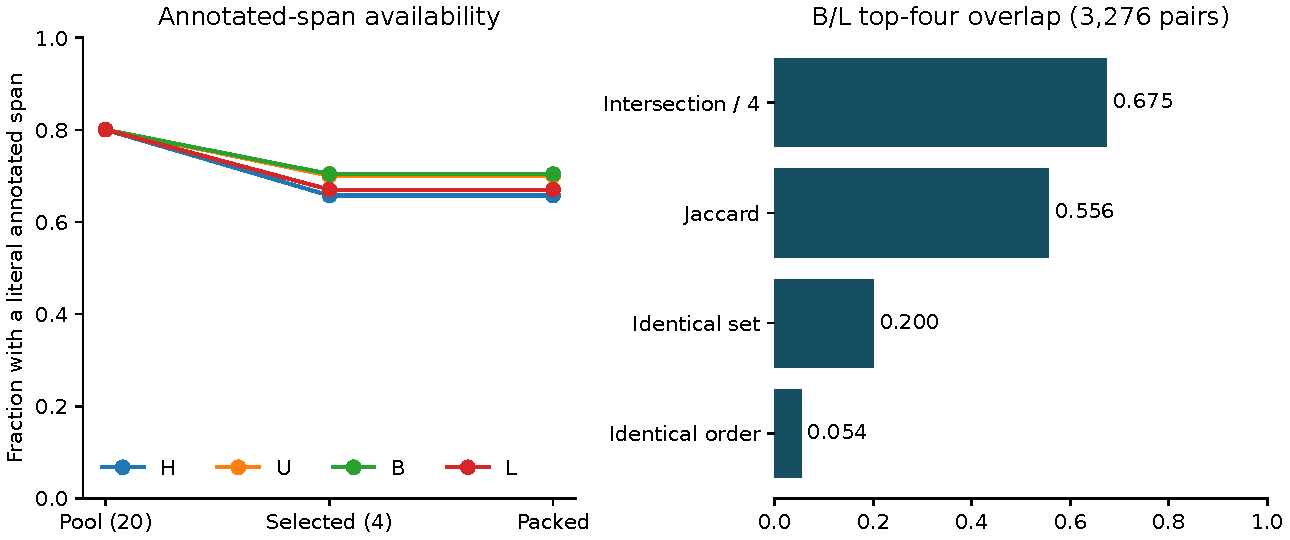
\includegraphics[width=\linewidth]{figures/study2_evidence_flow.pdf}
\caption{Left: fraction of cells with a literal annotated span in the 20-candidate pool, the selected four and the packed context. Right: top-four overlap between B and L over 3,276 paired cells.}\label{fig:flow}\end{figure}\FloatBarrier

\subsection{Grade composition and candidate-pool strata (post hoc)}
This post hoc analysis uses only the saved candidate pools, top-four rankings and generation-metric records; no model was invoked. File identities, all 8,736 ranking/metric keys, the full seed matrix and the saved overall and per-seed means were verified before the summaries were computed. Each B/L quantity is first averaged over its three paired seeds within a query--chunker cell and then uniformly over cells; H/U have one record per cell. The cells are dependent observations, and these summaries introduce no additional inferential tests.

Table~\ref{tab:gradecomposition2} reports selection shares for all three grades. To distinguish their contributions to graded NDCG, let
\[
C_g=\frac{1}{\mathrm{IDCG@4}}\sum_{i=1}^{4}\frac{\mathbf{1}\{g_i=g\}(2^g-1)}{\log_2(i+1)},\qquad g\in\{1,2\},
\]
with both components set to zero for zero IDCG. Thus $C_1+C_2=\mathrm{NDCG@4}$ for every record; the same identity holds for averages and paired differences. This is an arithmetic decomposition, not evidence of a causal optimization mechanism or semantic answer sufficiency.
\begin{table}[htbp]\centering\small
\caption{Top-four passage grade composition and normalized DCG contributions (post hoc). Shares are percentages of selected positions; $C_1+C_2$ equals NDCG@4. All 1,092 cells are included. NDCG components retain six decimals for this audit.}\label{tab:gradecomposition2}
\begin{tabular}{lrrrrrr}\toprule
Method & Grade 0 (\%) & Grade 1 (\%) & Grade 2 (\%) & $C_1$ & $C_2$ & NDCG@4\\\midrule
H & 48.12 & 27.22 & 24.66 & 0.215738 & 0.433897 & 0.649635\\
U & 46.11 & 27.50 & 26.40 & 0.216897 & 0.468632 & 0.685529\\
B & 45.96 & 27.82 & 26.23 & 0.219515 & 0.469391 & 0.688906\\
L & 50.82 & 24.19 & 24.98 & 0.184682 & 0.427070 & 0.611752\\
\bottomrule\end{tabular}\end{table}
\FloatBarrier

L selected fewer grade-1 passages than B (24.19\% versus 27.82\% of positions) and more grade-0 passages (50.82\% versus 45.96\%). Its $-0.077154$ NDCG difference from B decomposes into $-0.034832$ from grade~1 and $-0.042321$ from grade~2, or 45.1\% and 54.9\% of the observed drop. Relative to H, L selected slightly more grade-2 passages (24.98\% versus 24.66\%), yet its NDCG difference was $-0.037883$: $-0.031056$ from grade~1 and $-0.006828$ from grade~2 (82.0\% and 18.0\%). Selection counts ignore rank and pool-specific normalization, so this is consistent with the slightly higher binary grade-2 availability reported above.

The original 1,092 pools partition into 874 with a grade-2 candidate, 161 with grade-1 positives but no grade-2 candidate, and 57 with no positive grade. Tables~\ref{tab:strata2} and \ref{tab:dcgparts2} retain all three strata. L's NDCG difference from B is negative in both positive-grade strata; the grade-1-only stratum contributes $-0.021035$ to the population mean, or 27.3\% of the overall NDCG drop. Its response-F1 difference is positive within that stratum ($+0.73$ points), compared with $-0.39$ points in grade-2-available pools and $-0.34$ points in zero-grade pools. These post hoc differences do not establish a general relation between lexical retrieval grades and response quality. Zero-grade pools have NDCG zero by definition while their generated answers can still have nonzero token F1.
\begin{table}[htbp]\centering\small
\caption{Retrieval and response F1 within candidate-pool strata (post hoc). Response F1 is in points; NDCG@4 is on the 0--1 scale. B/L uniformly average the three paired seeds within each cell before cells are averaged.}\label{tab:strata2}
\begin{tabular}{lrlrr}\toprule
Pool stratum & Cells & Method & Response F1 & NDCG@4\\\midrule
Grade 2 available & 874 & H & 25.15 & 0.689\\
Grade 2 available & 874 & U & 25.36 & 0.728\\
Grade 2 available & 874 & B & 25.66 & 0.731\\
Grade 2 available & 874 & L & 25.27 & 0.661\\
\midrule
Grade 1 only & 161 & H & 18.55 & 0.666\\
Grade 1 only & 161 & U & 19.22 & 0.699\\
Grade 1 only & 161 & B & 18.26 & 0.704\\
Grade 1 only & 161 & L & 19.00 & 0.561\\
\midrule
Zero grade & 57 & H & 13.53 & 0.000\\
Zero grade & 57 & U & 17.19 & 0.000\\
Zero grade & 57 & B & 15.70 & 0.000\\
Zero grade & 57 & L & 15.36 & 0.000\\
\bottomrule\end{tabular}\end{table}
\FloatBarrier
\begin{table}[htbp]\centering\small
\caption{Within-stratum $L-B$ differences and additive NDCG decomposition (post hoc). F1 differences are in points. The three stratum differences, weighted by their cell counts divided by 1,092, reproduce the overall differences.}\label{tab:dcgparts2}
\begin{tabular}{lrrrrr}\toprule
Pool stratum & Cells & $\Delta$F1 & $\Delta$NDCG@4 & $\Delta C_1$ & $\Delta C_2$\\\midrule
All pools & 1092 & $-0.22$ & $-0.077154$ & $-0.034832$ & $-0.042321$\\
Grade 2 available & 874 & $-0.39$ & $-0.070116$ & $-0.017239$ & $-0.052878$\\
Grade 1 only & 161 & $+0.73$ & $-0.142674$ & $-0.142674$ & $+0.000000$\\
Zero grade & 57 & $-0.34$ & $+0.000000$ & $+0.000000$ & $+0.000000$\\
\bottomrule\end{tabular}\end{table}
\FloatBarrier

\subsection{Associations and generation records}
Table~\ref{tab:associations} reports document-level associations. For F1, NDCG@4 and generated-token length, each method's value is uniformly averaged over the same four chunkers and three paired training seeds within each document before subtracting B from L. The reported NDCG/F1 ($r=0.222451$, $\rho=0.176168$) and length/F1 ($r=-0.350358$, $\rho=-0.470186$) associations therefore use 273 paired $L-B$ document differences, each built from 12 cells. Grade-2 recall instead uses the 250 documents where it is defined; all other rows use 273. Predictors are $L-B$ differences, except overlap, which is the raw B/L overlap. Question difficulty, passage selection and output length can co-vary, so these associations do not identify a mechanism. Table~\ref{tab:generation} reports generation records.

The 273 reference agent utterances contain a mean of 16.31 tokens (median 14; 95th percentile 37) under the frozen answer-normalization and whitespace-tokenization rule; one becomes empty after normalization. Before normalization, their mean whitespace length is 17.58 tokens. These are lexical metric tokens, not generator subwords. Token F1 also has a mechanical length dependence: for nonempty normalized token sequences, $F1=2o/(n_{\mathrm{pred}}+n_{\mathrm{ref}})$, where $o$ is multiset overlap. With positive overlap, adding prediction tokens absent from the reference holds overlap and recall fixed while reducing precision and F1. This does not establish that a longer response is less supported or that shortening it would improve semantic correctness. The saved generation-length field counts generator subword tokens (including EOS when encountered), whereas F1 uses normalized whitespace-separated tokens; these units should not be conflated.

Table~\ref{tab:lexical} provides a post hoc, unit-matched diagnostic from the saved cleaned outputs. Generated answers average 63.80--65.60 normalized metric tokens, compared with 16.31 for the references. Precision and recall are computed per record from the same multiset overlap used in F1, then averaged; the F1 column independently reproduces the frozen means. An empty reference or prediction scores zero unless both are empty, matching the F1 empty-sequence convention. Mean F1 is the mean of record-level harmonic means, not the harmonic mean of the displayed mean precision and recall. These lexical diagnostics do not measure factual accuracy or support.
\begin{longtable}{lrrrrr}
\caption{Saved-output lexical diagnostics (post hoc). Length uses normalized whitespace metric tokens; precision and recall are percentages, and F1 is in points.}\label{tab:lexical}\\
\toprule Method & Records & Mean length & Precision & Recall & F1\\\midrule\endfirsthead
\toprule Method & Records & Mean length & Precision & Recall & F1\\\midrule\endhead
H & 1,092 & 63.80 & 17.94 & 51.65 & 23.57\\
U & 1,092 & 65.60 & 18.22 & 53.22 & 24.03\\
B & 3,276 & 64.43 & 18.23 & 52.90 & 24.05\\
L & 3,276 & 64.57 & 18.09 & 52.80 & 23.83\\\bottomrule
\end{longtable}
\begin{table}[htbp]\centering\small
\caption{Document-level associations with the $L-B$ response-F1 difference (exploratory). Predictors are $L-B$ differences, except top-four overlap, which is the raw B/L overlap.}\label{tab:associations}
\begin{tabular}{lrrr}\toprule
Predictor & N & Pearson $r$ & Spearman $\rho$\\\midrule
NDCG@4 & 273 & 0.22 & 0.18\\
Grade-2 recall & 250 & 0.26 & 0.23\\
Selected grade-2 count & 273 & 0.25 & 0.22\\
Selected annotated span & 273 & 0.29 & 0.23\\
Packed annotated span & 273 & 0.29 & 0.23\\
Packed full target & 273 & 0.09 & 0.07\\
Generated tokens & 273 & $-$0.35 & $-$0.47\\
Length capped & 273 & $-$0.05 & $-$0.07\\
Top-four overlap & 273 & $-$0.06 & $-$0.07\\
\bottomrule\end{tabular}\end{table}

\begin{table}[htbp]\centering\small
\caption{Study 2 generation records. Truncated refers to the context; capped to the 512-token output limit. Legacy 2 counts records with the invalid historical prompt-length value (Section~\ref{sec:s5}).}\label{tab:generation}
\begin{tabular}{lrrrrr}\toprule
Method & Records & Mean tokens & Truncated & Capped & Legacy 2\\\midrule
H & 1092 & 88.5 & 1 & 0 & 745\\
U & 1092 & 91.3 & 1 & 0 & 745\\
B & 3276 & 89.8 & 2 & 1 & 2234\\
L & 3276 & 90.0 & 1 & 1 & 2234\\
\bottomrule\end{tabular}\end{table}
\FloatBarrier
The saved prompt-length field contains the value 2 in 5,958 records (745 of 1,092 H, 745 of 1,092 U, 2,234 of 3,276 B and 2,234 of 3,276 L) because a legacy helper counted a returned mapping rather than its token dimension. These values are not prompt lengths. The recorded compatibility audit reconstructed all 8,736 planned packing cases from the frozen rankings with Qwen/Qwen3.5-9B's pinned tokenizer, including the 5,958 cases whose answers had already been recovered. It found a maximum corrected and rendered input length of 1,536, no count mismatches, and five contexts requiring truncation (one H, one U, two B and one L). None of those five had been generated at the time of the repair, so no completed answer required regeneration. The final saved truncation flags also total five. These figures come from the recorded full-matrix budget audit; no new tokenizer replay was performed. Tensor-width checks enforced the limit during generation, and the saved records were not modified. Reproduction should use the executed (repaired) generation code rather than the older packing helper.

\section{Cost, environment and technical fixes}\label{supp:cost}
\subsection{Compute}
Tables~\ref{tab:trainingcost}--\ref{tab:retrievalcost} report recorded component measurements. The Study~2 allocation ledger totals 46,280 seconds (12.86 A100-hours), 7.14 hours under the planned 20-hour budget. It includes loading, I/O, failed attempts and retries, and excludes development smoke tests and earlier project compute. Training timers may cover only a resumed session of a job and should not be summed as a GPU-hour estimate.
\begin{table}[htbp]\centering\small
\caption{All 12 grid and six refit jobs. Passes = group draws divided by available groups. Session time may cover only the last resumed session of a job.}\label{tab:trainingcost}
\begin{tabular}{lrrrrrrr}\toprule
Stage & Method & Seed & LR & Updates & Groups & Passes & Session (s)\\\midrule
grid & B & 20260904 & $5\times10^{-5}$ & 227 & 2103 & 0.43 & 352.1\\
grid & B & 20260904 & $5\times10^{-5}$ & 454 & 2103 & 0.86 & 700.1\\
grid & B & 20260904 & $5\times10^{-5}$ & 681 & 2103 & 1.30 & 1048.0\\
grid & B & 20260904 & $10^{-4}$ & 227 & 2103 & 0.43 & 351.6\\
grid & B & 20260904 & $10^{-4}$ & 454 & 2103 & 0.86 & 397.2\\
grid & B & 20260904 & $10^{-4}$ & 681 & 2103 & 1.30 & 1048.9\\
grid & L & 20260904 & $5\times10^{-5}$ & 227 & 943 & 0.96 & 345.5\\
grid & L & 20260904 & $5\times10^{-5}$ & 454 & 943 & 1.93 & 692.0\\
grid & L & 20260904 & $5\times10^{-5}$ & 681 & 943 & 2.89 & 1040.3\\
grid & L & 20260904 & $10^{-4}$ & 227 & 943 & 0.96 & 346.6\\
grid & L & 20260904 & $10^{-4}$ & 454 & 943 & 1.93 & 694.4\\
grid & L & 20260904 & $10^{-4}$ & 681 & 943 & 2.89 & 1041.3\\
refit & B & 20260904 & $10^{-4}$ & 431 & 4019 & 0.43 & 670.1\\
refit & B & 20260905 & $10^{-4}$ & 431 & 4019 & 0.43 & 670.4\\
refit & B & 20260906 & $10^{-4}$ & 431 & 4019 & 0.43 & 672.5\\
refit & L & 20260904 & $10^{-4}$ & 431 & 1799 & 0.96 & 670.2\\
refit & L & 20260905 & $10^{-4}$ & 431 & 1799 & 0.96 & 669.5\\
refit & L & 20260906 & $10^{-4}$ & 431 & 1799 & 0.96 & 669.2\\
\bottomrule\end{tabular}\end{table}
\FloatBarrier
\begin{table}[htbp]\centering\small
\caption{Batched reranker scoring (batch size 32). Pairs and scoring seconds cover all batches; pairs/s excludes the first 32-pair batch and uses 21,808 pairs per instance. Loading is separate. These are synchronized forward-pass measurements, not request latency.}\label{tab:rerankcost}
\begin{tabular}{lrrrrr}\toprule
Instance & Pairs & Base load (s) & Adapter load (s) & Scoring (s) & Pairs/s\\\midrule
U & 21840 & 1.05 & 0.00 & 133.0 & 164.2\\
B, seed 20260904 & 21840 & 1.02 & 0.44 & 238.2 & 91.7\\
B, seed 20260905 & 21840 & 1.03 & 0.47 & 238.3 & 91.7\\
B, seed 20260906 & 21840 & 1.07 & 0.44 & 238.3 & 91.7\\
L, seed 20260904 & 21840 & 1.03 & 0.44 & 238.3 & 91.7\\
L, seed 20260905 & 21840 & 1.04 & 0.45 & 238.3 & 91.6\\
L, seed 20260906 & 21840 & 1.03 & 0.46 & 238.3 & 91.6\\
\bottomrule\end{tabular}\end{table}
\FloatBarrier
\begin{table}[htbp]\centering\small
\caption{Retrieval component timings per query--chunker cell (milliseconds). Index construction and model loading are excluded.}\label{tab:retrievalcost}
\begin{tabular}{lrrrr}\toprule
Component & Cells & Mean & Median & 95th pct\\\midrule
BM25 & 1092 & 87.20 & 77.35 & 206.35\\
Dense & 1092 & 14.50 & 14.38 & 15.53\\
Fusion & 1092 & 0.06 & 0.06 & 0.07\\
Total & 1092 & 101.76 & 91.75 & 221.22\\
\bottomrule\end{tabular}\end{table}
\FloatBarrier
Each reranker instance scored the same 21,840 query--passage pairs at batch size 32. The recorded steady scoring rate excludes the first 32-pair batch, so its denominator is 21,808 pairs per instance, not 21,840. The rates are 164.23 pairs/s for U, 91.65--91.67 for the three B adapters, and 91.64--91.66 for the three L adapters. Pooling timed scoring seconds within method gives 91.66 and 91.65 pairs/s for B and L, respectively (65,424 steady pairs each; 65,520 total pairs per adapted method and 131,040 adapted pairs in total). Base loading took 1.05 seconds for U, 1.02--1.07 for B and 1.03--1.04 for L; adapter loading additionally took 0.44--0.47 seconds for B and 0.44--0.46 for L. Scoring timers surround synchronized GPU forward passes, after CPU tokenization and transfer, and exclude loading, full retrieval, generation and other service overheads. These offline component timings are not end-to-end serving latency or evidence that the measured ratios would hold in another deployment.
The final generation session processed 300 records in 75 batches and produced 29,912 tokens in 614.5 seconds (48.7 tokens/s; 0.49 records/s), with 231.4 seconds of model loading and a peak allocation of 18.2 GiB. These values describe that session only, not the full 8,736-record run, per-request latency or a matched serving comparison. No time-to-first-token, network, queueing or deployment measurements are available.

\subsection{Software environment and technical fixes}
The recorded Study~2 environment is Python 3.13.15, PyTorch 2.11.0+cu128, Transformers 5.16.1, PEFT 0.20.0, Accelerate 1.14.0, NumPy 2.1.3 and Hugging Face Hub 1.28.0 on an NVIDIA A100-SXM4-40GB, with faiss-cpu 1.14.3, langchain-text-splitters 0.3.11, rank-bm25 0.2.2, sentence-transformers 3.4.1 and spaCy 3.8.14 for retrieval. Newer default environments may not reproduce the experiment exactly.

Two development smoke tests failed before the full run: one at a split-membership precheck before model loading, and one before any optimizer update because an unused dependency (torchao) was incompatible. After removing that dependency, the next smoke test succeeded. The full-run recovery scripts, the generation token-budget audit and the finalization scripts are part of the reproduction dependencies. The completed outputs passed 28 finalization, recovery and contract tests and a 17-check final verification.

\section{Reproduction dependencies}\label{supp:repro}
The public companion provides selected source, configuration, pre-execution protocol and aggregate results. The first release (v1.0.0) is archived at DOI \href{https://doi.org/10.5281/zenodo.22695835}{\mbox{10.5281/zenodo.22695835}}; subsequent documentation is identified as release v1.0.1 at \url{https://github.com/zukhriddingit/chunkrag-reranking-study}. The protocol was fixed before comparative Doc2Dial outcomes but released afterward; it is not a public preregistration. Code/configuration use Apache-2.0 and designated author-owned aggregates/documentation use CC-BY-4.0, as assigned per file; these licenses do not replace third-party terms.

\begin{longtable}{P{0.24\linewidth}P{0.34\linewidth}P{0.34\linewidth}}
\caption{Artifact access and replay limits of the current companion.}\label{tab:access}\\
\toprule Artifact & Current access & Consequence\\\midrule\endfirsthead
\toprule Artifact & Current access & Consequence\\\midrule\endhead
Dataset text & Upstream TechQA-RAG-Eval (card: Apache-2.0) and IBM Doc2Dial (card: CC-BY-3.0); pinned versions in \supp{S2}{supp:impl} & Dataset availability does not reproduce the selected cases or trained adapters.\\
Exact splits and turn selections & Not included in the companion; deterministic hash rule and salt specified here & ID-only exports can improve auditability without redistributing dialogue/answer text; a local candidate is not a public release.\\
Saved rankings, generations and per-record metrics & Not included in the companion & Aggregate checks are possible; independent raw-record recomputation requires the saved records. No claim of an established blanket redistribution prohibition is made.\\
Six final adapters & Not included; base model and revision identified & Published weights do not recreate our fitted adapters. No public adapter endpoint or on-request access mechanism is promised.\\
Training/evaluation and recovery code & Selected source is included; complete executed repair/runtime dependencies remain necessary & The companion is not a one-command or complete model-experiment replay package.\\\bottomrule
\end{longtable}

Upstream cards are \url{https://huggingface.co/datasets/nvidia/TechQA-RAG-Eval} and \url{https://huggingface.co/datasets/IBM/doc2dial}. These exclusions reflect release scope; the paper does not establish that benchmark identifiers, non-human outputs or adapter weights are legally unshareable. Any expanded release should identify the exact files, preserve the relevant notices and document its access conditions.
